\chapter{The Level 1 trigger upgrade} % 
\label{sec:triggerUpgrade}

During Run 2, the LHC has provided collisions at energy of 13\TeV~and at up 
to a peak luminosity of $14\times10^{33}cm^{-2}s^{-1}$, marking a signifcant increase
in peak energy and luminosity provided during Run 1 (8\TeV~and $7\times10^{33}cm^{-2}s^{-1}$).
At 25ns bunch spacing an average of 25 simlutaneous interactions are produced.
The instantaneous luminosity and pileup provide a challenging environment for the L1 trigger system
during Run 2, exceeding design specifications. The rate into the HLT must 
remain at 100kHz. Simply increasing thresholds on the L1 trigger seeds would imply
unacceptable inefficiencies for electroweak physics and \TeV~ scale searches
at CMS and so the L1 trigger system, and associated algorithms, must be upgraded. 

In the following, the upgrades to the L1 calorimetric trigger system and the 
associated L1 jet algorithm are discussed. The muon trigger system 
and upgrades to the algorithms for identification of other physics objects for the L1 trigger are discussed 
in~\cite{ele_algo,tau_algo,muon_algo}.


\section{Legacy system and upgrade}

The Global Calorimeter Trigger (GCT) was used during Run 1 to find jets, electrons and photons and to 
compute global energy sums \cite{gct}. The trigger system takes input from trigger towers (TT) corresponding to $5\times5$ ECAL crystals 
and an identical area in the HCAL. These are grouped into $4\times4$ \emph{regions} which form the input for physics object and
reconstruction algorithms. These inputs are provided by Trigger Primitive Generators (TPGs). 
Due to hardware limitations the detector is split into 16 
regions which are processed by separate Regional Calorimetric Triggers (RCTs) to form candidates and sum 
energies. The RCTs must share information to account for features which occur at boundaries between 
them. The information from the RCTs is combined in the GCT which computes global quantities and sorts 
the jets before sending to the Global Trigger which also receives the Muon trigger
information and makes the final trigger decision. 

The upgrade of the GCT was carried out in two stages. The first stage
Upgrade Calorimetric Trigger (UCT) was used for data taking during 2015
and used updated firmware and algorithms to allow improved pileup subtraction (PUS)
and improved jet and object identification \cite{uct}. In the second stage the 
architecture was entirely replaced by the Time Multiplexed Trigger (TMT) 
to allow \emph{time multiplexing} whereby each
event is processed entirely within one card using the full trigger tower granularity. 

\section{The Time Multiplexed Trigger architecture}

The TMT uses two processing layers. The first, layer 1, performs
pre-processing and data formatting using 18 CTP7 cards \cite{mp7}. Each card requires
only a regional view of the detector and performs local operations such as summing 
ECAL and HCAL transverse energies. The data for each event is combined and transmitted to 
a single node in the layer 2, an Imperial Master Processor Virtex-7 (MP7) card. 
The MP7 is a high performance 0.92Tb/s + 0.92Tb/s (input + output rate) all-optical processor \cite{mp7}
with sufficient data rate for the entire calorimeter to be processed in a single card. The data 
from the 9 layer 2 nodes is sent to a demultiplexer board (also an MP7) to be formated before
the data is sent to the Global Trigger.

The difference between the GCT and TMT architectures is shown in Figure~\ref{tmux}. 
In the TMT architecture, data is buffered and retransmitted to the first node (on layer 2)
over 9 bunch crossings to allow the entire event to be processed on one card. This
removes the need for a large number of links between cards and allows the full trigger
tower granularity to be used. The increase in granularity compared to the GCT is
illustrated in Figure~\ref{fig:inputres}. 

\begin{figure}

\centering
    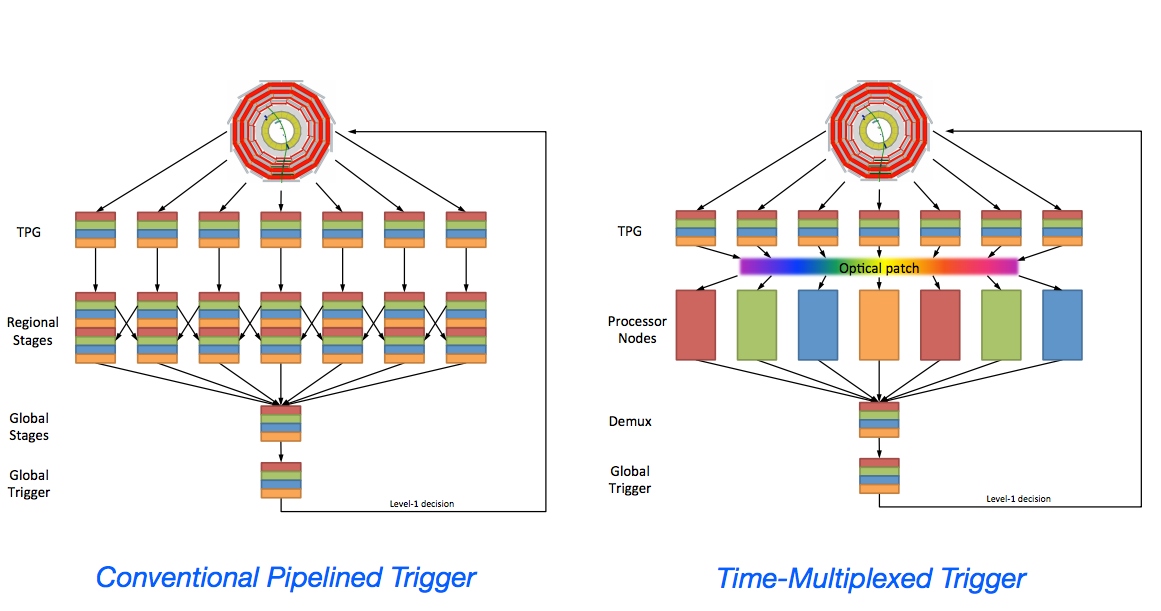
\includegraphics[width=0.9\textwidth]{./Figures/triggerUpgrade/tmux}
  \caption{Comparison of the GCT (left) and TMT architectures (right) showing the flow of information
  to the final global decision. The colours indicate the data from each bunch crossing. \cite{tmt}}
  \label{tmux}
\end{figure}

\begin{figure}
\centering
\subfigure[Input resolution: GCT]{
\includegraphics[width=0.35\textwidth]{./Figures/triggerUpgrade/L1inputreslegacy.png}\label{subfig:inputlegacy}} \quad
\subfigure[Input resolution: stage 2 upgrade]{
\includegraphics[width=0.35\textwidth]{./Figures/triggerUpgrade/L1inputresupgrade.png}\label{subfig:inputupgrade}} 
\caption{A representation of the CMS collaboration logo digitised with the input resolution of the L1 calorimeter trigger up to 
\etaabs~$< 3$ using (a) the legacy system ($18 \times 14$ pixels) and (b) the stage 2 upgrade ($72 \times 56$ pixels).}
\label{fig:inputres}
\end{figure}

\section{L1 jet algorithm}
\label{algo}

The increase in pileup and luminosity in Run 2 makes triggering with jets
significantly more challenging than during Run 1. To maintain sensitivity to
new physics the new algorithm must allow high efficiencies and
low rates even for high pileup scenarios.

The TMT architecture provides several advantages over the GCT system which can be 
exploited in designing the jet algorithm, including significantly increased processing power
and granularity (enhanced by factor 16). This allows more flexible algorithms, which can 
exploit smaller features than previously accessible, to be defined. This is exploited in the 
use of an improved jet clustering (described in Section~\ref{sec:jet_algo}) algorithm as well as 
online PUS techniques (described in Section~\ref{sec:pileup_algo}) in the upgrade jet 
identification and reconstruction algorithm.

\subsection{L1 jet clustering}
\label{sec:jet_algo}
The GCT algorithm uses a $3\times3$ calorimeter region sliding jet window with a central seed 
to reconstruction jets in the range $|\eta| < 5$. The algorithm scans the calorimeter in increments
of regions and clusters a jet if the energy in the central seed region is greater than 
both $5\GeV$ and each of the eight bordering regions. The threshold of $5\GeV$ was added during 
the 2012 8\TeV run, when the number of pileup interactions increased, to remove soft pileup jets.
The $12\times12$ TT ($\Delta\eta\times\Delta\phi = 1.04\times1.04$) jet size corresponds 
approximately to $R=0.5$ for the anti$k_T$ jet algorithm used in offline reconstruction.

The jet algorithm used for the stage 2 upgrade similarly uses a sliding window algorithm. This
is composed of $9\times9$ TTs ($\Delta\eta\times\Delta\phi = 0.78\times0.78$), corresponding 
to the $R=0.4$ used in Run 2. The use of an odd number of trigger towers ensures a central 
seed tower can be defined. 

In order to ensure that jets do not overlap, the seed tower is required to meet the conditions
shown in Figure~\ref{mask}. The veto conditions are asymmetric along the diagonal to ensure  
that TTs with the same energy cannot veto one another. These veto conditions ensure that there 
is no double counting of overlapping jets. An inefficiency may be expected 
as one jet may veto another which itself vetoes a third (\emph{chain} veto). However, this effect was found to 
introduce a negligible (~0.1\%) inefficiency. A central seed threshold may be 
additionally required to reconstruct a jet, as discussed in section~\ref{sec:seed_thresh}. 

If a seed passes the veto requirements a jet is defined with a position given
by the seed position and an energy given by the total energy of the towers. The position is
given by that of the seed as jets tend to be boosted objects with an energy deposited in
a small central area. Note that the L1 jets are massless such that $\pt = \Et$.

\begin{figure}
\centering
    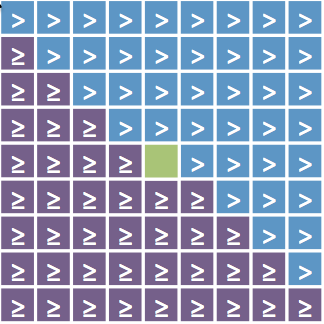
\includegraphics[width=0.5\textwidth]{./Figures/triggerUpgrade/mask.png}
  \caption{The $9\times9$ veto conditions used to define jets. The inequalities ensure
  jet energies are not double counted}
  \label{mask}
\end{figure}

\subsection{Comparison with offline jet reconstruction}

An evaluation of the performance of the L1 jet algorithm can be made by comparing
the results of jet finding with the offline reconstruction algorithm used by 
most CMS analyses during Run 2, anti-$k_T$ with a distance
parameter of 0.4, described in Section~\ref{sec:jet_reco}. 

The trigger tower deposits were generated with a simulated sample of top pair-production \footnote{In this section all simulated samples used have conditions 
of $\sqrt(s) = 13TeV$, bunch spacing $50ns$ and pileup Gaussian distributed around $40$ simultaneous interactions.} 
due to the plentiful sample of jets produced in this process. The anti-$k_T$ algorithm is run over the same inputs as
used for the L1 algorithm using the \FASTJET package.

A comparison between the predictions of both algorithms is shown for several important jet variables in 
Figure~\ref{fig:jet_l1s2_compak4} for the leading and fourth jet. In general, excellent agreement is observed, however,
small differences can be seen at high $|\eta|$ and low $p_T$. This is due to the ability 
of the anti$k_T$ algorithm to reconstruct smaller jet radii while the L1 jet
algorithm size is fixed.


\begin{figure}
\centering
    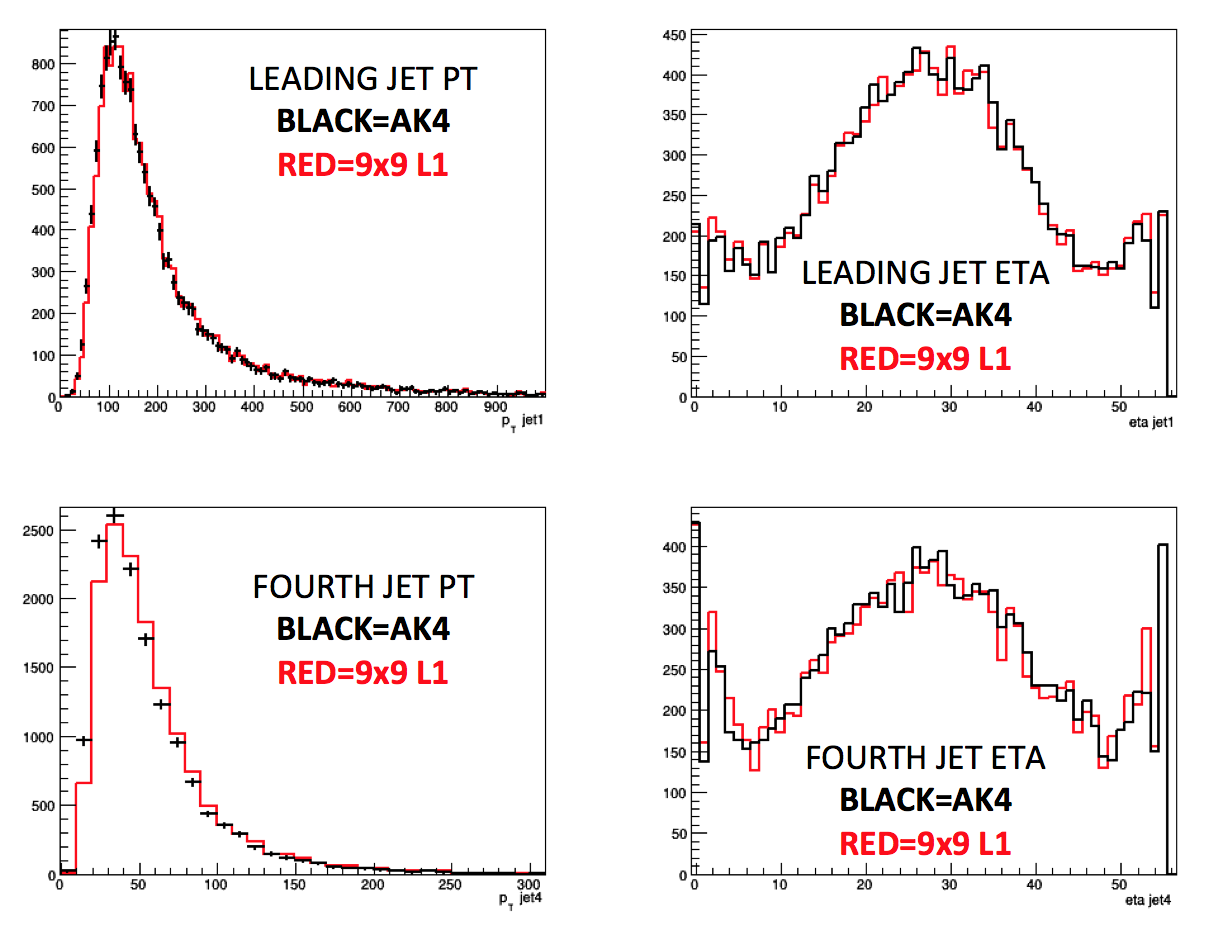
\includegraphics[width=0.8\textwidth]{./Figures/triggerUpgrade/jet_l1s2_compak4}
  \caption{Comparison of the L1 jet finding algorithm with the anti-kt algorithm using
  trigger tower inputs. Distributions of \pt~and $\eta$ are shown for the leading and fourth
  jet.}
  \label{fig:jet_l1s2_compak4}
\end{figure}  
\subsection{Energy sums}

In addition to jet reconstruction the L1 calorimeter trigger must also build energy sums. 
These can be made using both the jets and individual calorimeter deposits, analogously to
the offline quantities. The baseline quantities that are constructed are

\begin{itemize}
\item L1 total \Et -- the scalar sum the $E_T$ of all calorimeter TTs;
\item L1 \met -- the inverse vector sum of the $E_T$ of all calorimeter TTs;
\item L1 \scalht -- the scalar sum of all L1 jet \pt;
\item L1 \mht -- the inverse vector sum of all L1 jet \pt.
\end{itemize}

The quantities made using L1 jets require a minimum \Lonept of 20\GeV. As will be discussed in 
Section~\ref{sec:trig_perf}, this requirement provides additional robustness against soft
jet reconstructed from detector noise or pileup. Additional quantities based 
on jets and/or energy sums may also be defined. A study of the use of one such variable is detailed in Section ??.

\section{Pileup subtraction}
\label{sec:pileup_algo}
Simultaneous soft interactions will cause additional energy to be deposited throughout
the detector. This will be approximately isotropically distributed ($\sim1\GeV$ per unit area), however, variations
in detector response as well as the profile of pileup events can cause $\eta$ and,
to a lesser extent $\phi$ dependence. In addition, event-by-event fluctuations in the distribution 
and magnitude of the pileup deposits can greatly affect calorimeter objects. 
The effect of pileup can be to increase the energy of jets associated to the hard 
scatter as well as causing additional pileup jets
to be clustered entirely from pileup energy deposits.

Pileup subtraction at L1 aims to remove contributions from pileup such that the trigger
decision is unbiased by the simultaneous interactions. Changes during running
to detector response, beam conditions and the random nature of pileup necessitate an event-by-event
estimation and mitigation of the pileup contribution. This must be done using only the calorimeter as 
tracker information is unavailable at L1. Several methods that meet the stringent latency requirement
are discussed in this Section. These rely on both global event estimations of pileup as well as 
local methods that can account for anisotropy in the pileup distribution, while being more susceptible 
to statistical fluctuations, to perform pileup correction and reject pileup jets.

\subsection{Jet area method}%Global $\boldsymbol{\rho}$}

The jet area method uses the jets themselves to estimate the \rhoP~(\rhoP) using
the median energy density of all jets in the event, defined as \rhoG~\cite{jet_area}. 
The main assumptions in this method are that the pileup distribution is independent of $\eta$ and $\phi$,  
and the number of pileup jets must be much larger than those from the hard scatter. Using \rhoG, 
a correction to each jet can be made

\begin{equation}
\label{equ:global_rho}
p_{Tj}^{\text{subtracted}} = p_{Tj}^{\text{raw}} - \rho_{\text{global}} \cdot A_j,
\end{equation}


where $A_j$ is the area of the jet $\Delta\phi\Delta\eta(\eta)$ which is dependant on $\eta$ due 
to variation in the jet tower size. If $\rho \cdot A_j > p_{Tj}^{\text{raw}}$ the jet is discarded. 
Figure~\ref{fig:medianNint} shows a strong linear dependence between \rhoG~and the number of interactions for
minimum bias events. The non-zero intercept is caused by contamination from jets from the hard scatter.
The \rhoG~subtraction may be amended to account for $\eta$ dependence in the pileup by 
dividing the calorimeter into strips of phi and calculating the median $\rho$ for jets in each 
strip. However, this local $\rho$ significantly adds to the latency in the PUS and may 
be less robust as fewer jets can be sampled in each $\eta$ slice. 

\begin{figure}
\centering
    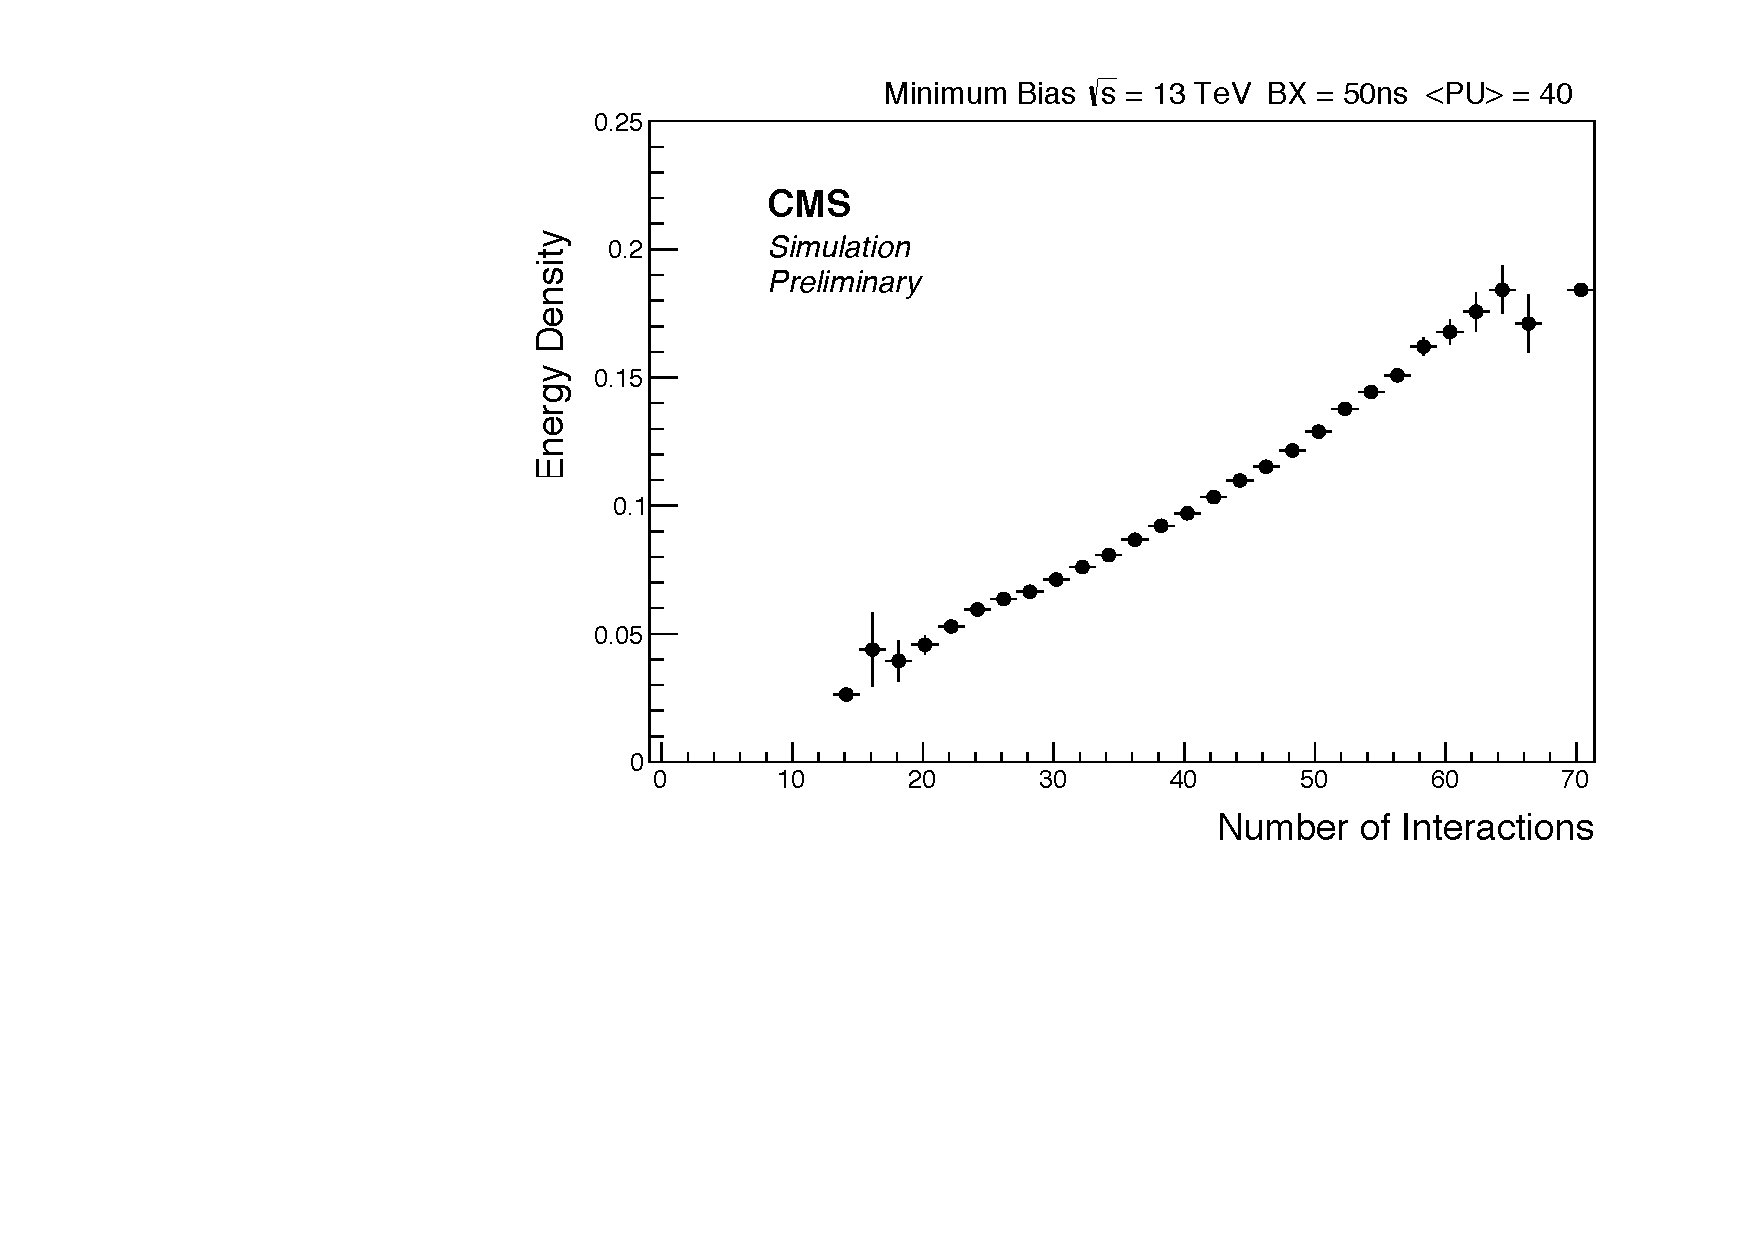
\includegraphics[width=0.8\textwidth]{./Figures/triggerUpgrade/median}
  \caption{Dependence of \rhoG (arbitrary units) on the number of interactions}
  \label{fig:medianNint}
\end{figure}  

\subsection{Doughnut subtraction}
\begin{figure}
\centering
    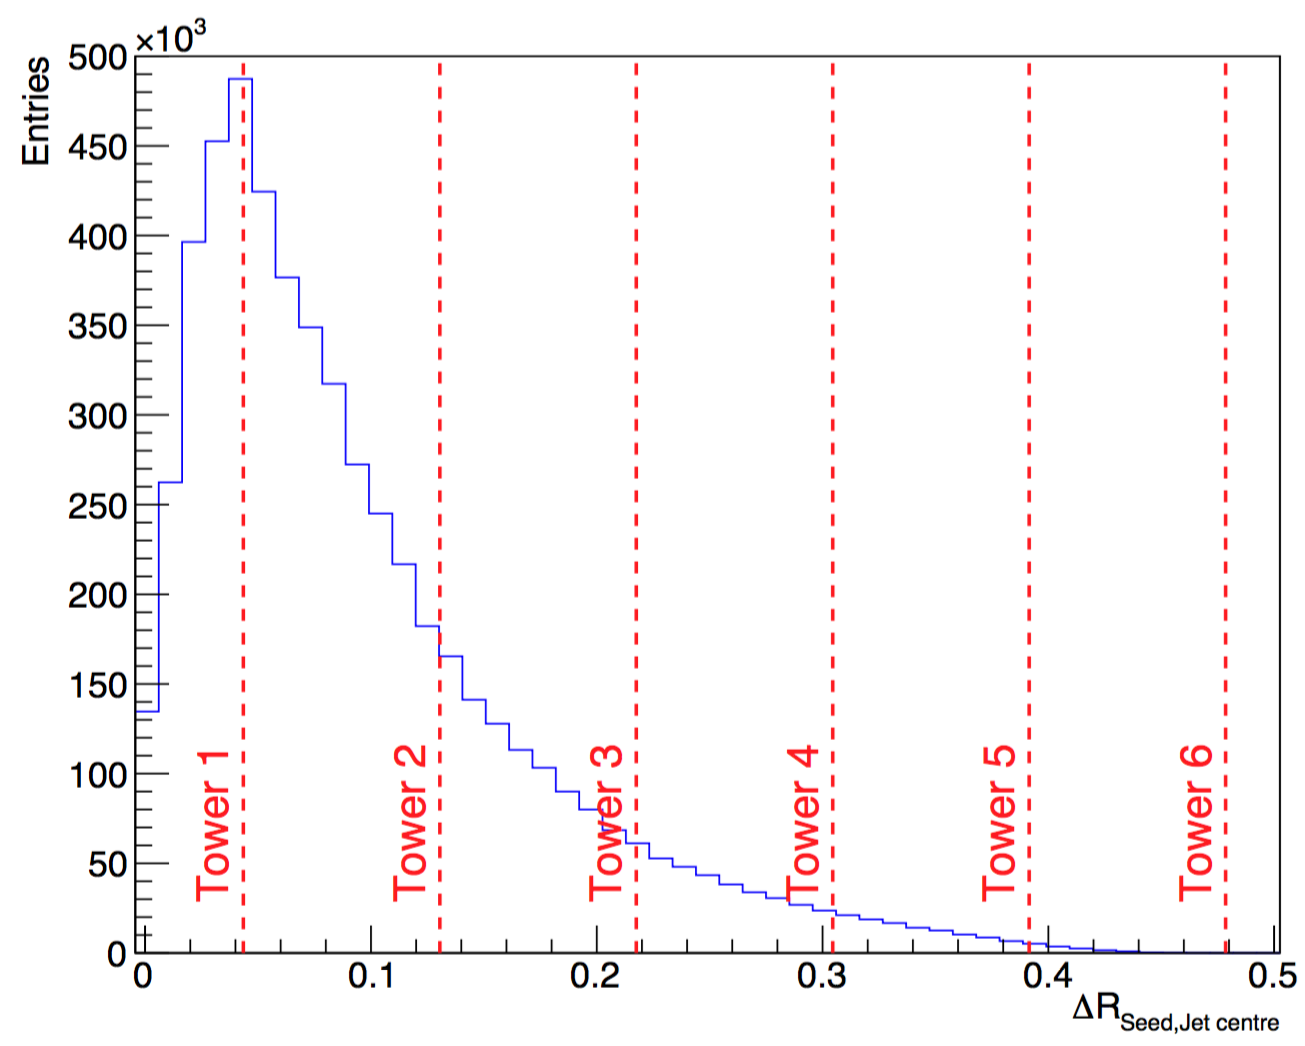
\includegraphics[width=0.8\textwidth]{./Figures/triggerUpgrade/deltaR2}
  \caption{$\Delta R$ distribution between the seed and constituent TTs using data from Run 1.}
  \label{fig:deltaR2}
\end{figure}  


Doughnut subtraction makes use of the area around the jet to sample the local pile-up
energy density in order to correct (or reject) each jet and has been previously proposed
for use during heavy ion collisions~\cite{doughnut}. The energy contribution from the jet
itself is negligible outside the $9\times9$ ring as shown in Figure~\ref{fig:deltaR2}. 
For doughnut subtraction the transverse energy density is sampled by taking four strips around 
the jet as shown in Figure~\ref{fig:donut}. The strips are ordered according to energy density,
and the median two strips taken. The pileup energy density estimated from the 
energy density of the median two strips. This \rhoD is used to correct the
jet analogously to Equation~\ref{equ:global_rho}. Using the median strips to estimate \rhoP~allows
contributions from nearby jets to be removed such that any bias due to such jets is 
mitigated.
% This is illustrated in Figure~\ref{}. 
% If all strips are taken in calculating $\rho_{pileup}$, the estimation is biased for non-isolated jets, 
% however, by taking the median two strips this bias is mitigated.
Unlike global subtraction, doughnut subtraction allows local variations in \rhoP~to be 
included, however, it is significantly more susceptible to statistical fluctuations due to the 
reasonably small area sampled. An extension, \emph{chunky} doughnut, shown in Figure~\ref{fig:chunkyDonut},
uses enlarged strips to sample three times the area. The dependence of the number of interactions
with the energy density for the chunky doughnut pileup estimation (\rhoC) is shown in Figure~\ref{fig:threestripNint}.

\begin{figure}
\hfill
\subfigure[Doughnut rings\label{fig:donut}]{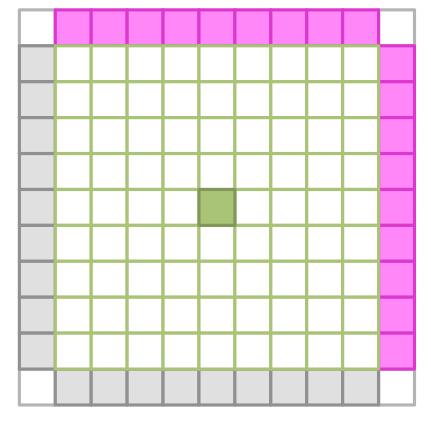
\includegraphics[width=7cm]{./Figures/triggerUpgrade/donut}}
\hfill
\subfigure[Chunky doughnut rings\label{fig:chunkyDonut}]{
\includegraphics[width=7cm]{./Figures/triggerUpgrade/chunkyDonut}}
\hfill
\caption{The rings used to sample the local pileup energy density for the doughnut (left) and chunky doughnut (right)
PUS. The median two strips (in energy density) are used in each case.}
\end{figure}

\begin{figure}
\centering
    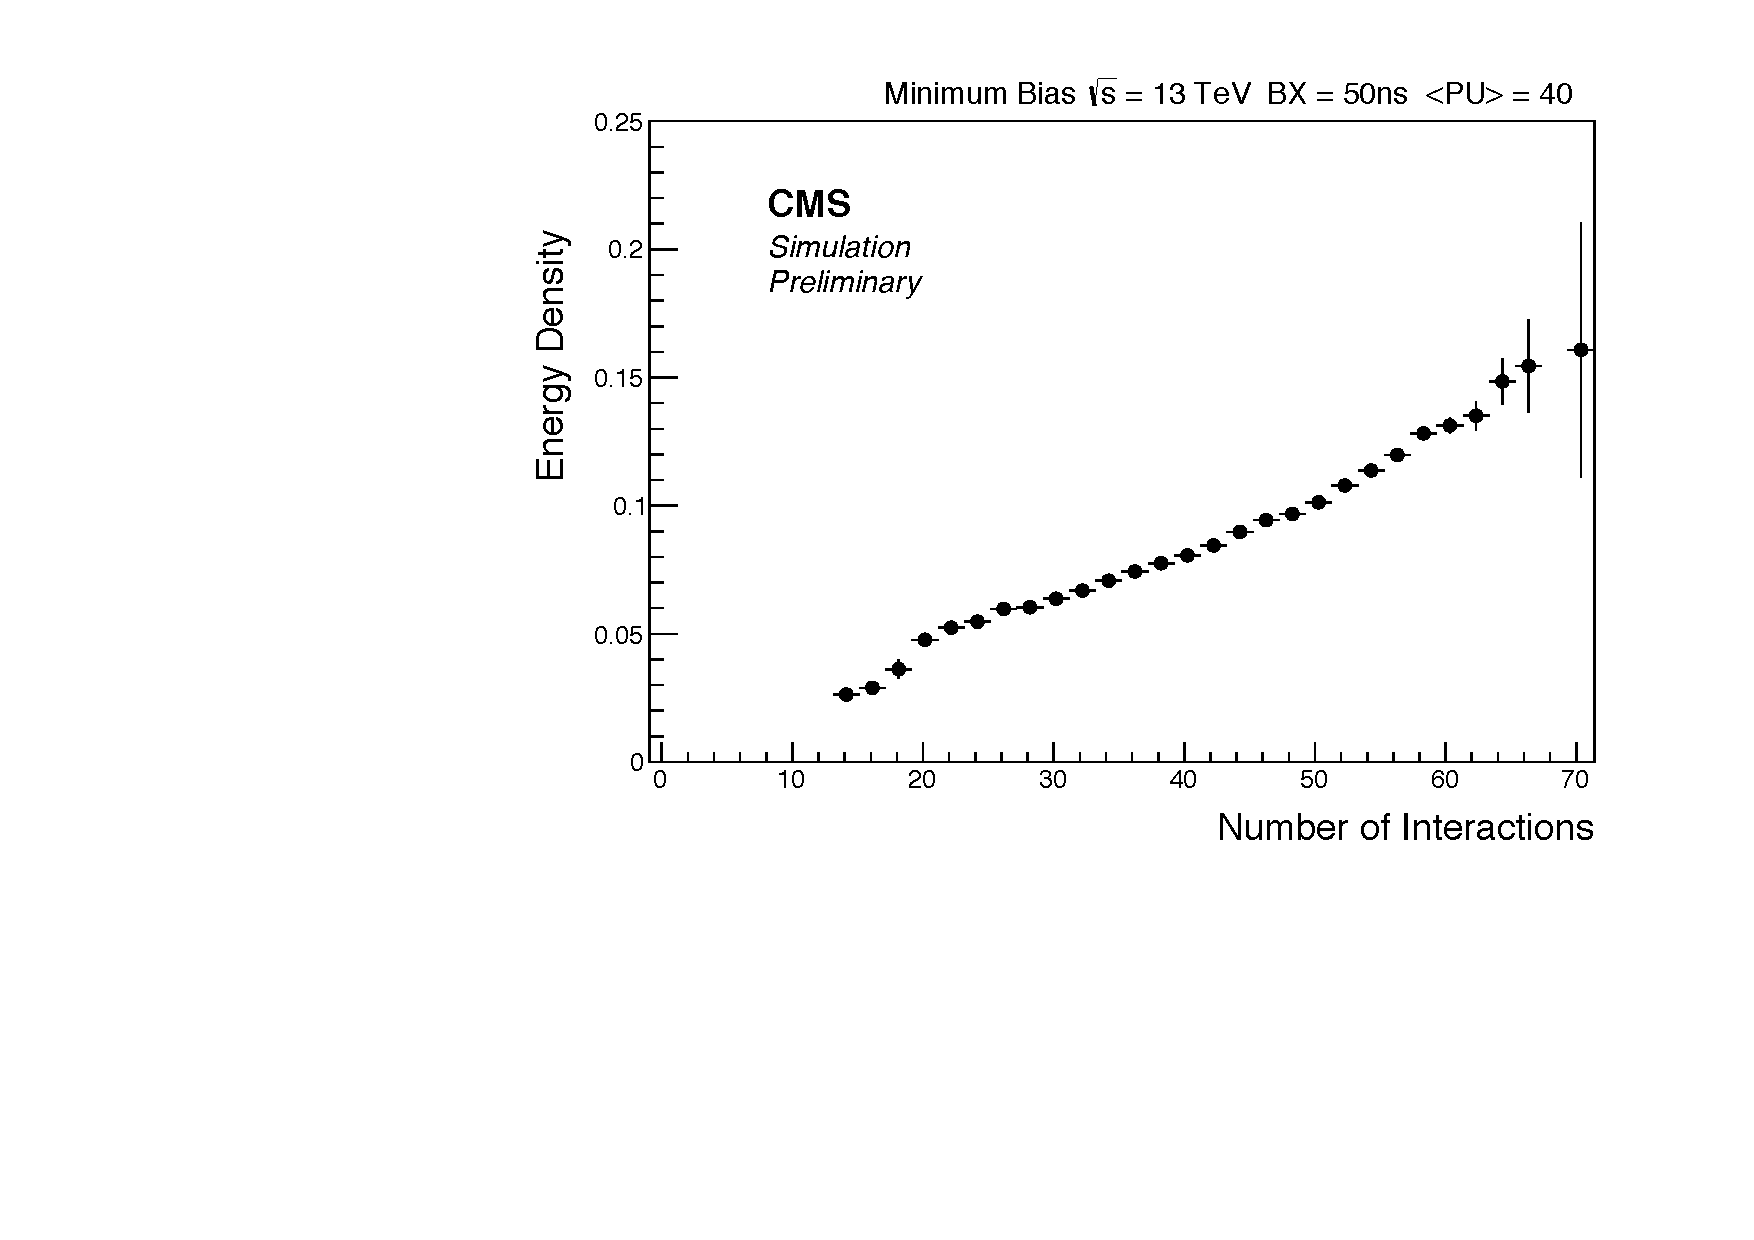
\includegraphics[width=0.8\textwidth]{./Figures/triggerUpgrade/threestrips}
  \caption{Dependence of the \rhoC (arbitrary units) on the number of interactions}
  \label{fig:threestripNint}
\end{figure}  

\subsection{Seed threshold and zero suppression}
\label{sec:seed_thresh}
The requirement of a seed threshold for the central tower when reconstructing a jet
provides a powerful rejection of pileup jets. This takes advantage of the generally 
diffuser energy deposition for pileup jets compared to jets originating from 
the hard scatter. This does not allow the contamination in non pileup jets to be corrected
but can be used in conjunction with other PUS techniques. The global
$\rho$ subtraction is incompatible with a seed threshold as this technique relies
on reconstructing substantially more pileup jets than those from the hard scatter. 
This problem may be addressed by using a separate collection with no seed threshold
to calculate $\rhoG$, however, latency constraints do not permit this for the L1 trigger.

Zero suppression is a rudimentary form of pileup correction whereby only towers with
energy deposition above a given threshold are included in the reconstruction of each jet.
This cannot be easily adapted to a range of pileup regimes but provides a simple baseline 
for assessing more complex algorithms. Zero suppression may also be used in conjunction
with other pileup correction techniques. 

The thresholds used for the seed and zero suppression may be $\eta$ (or even $\phi$) dependant, however,
such variable thresholds are not considered in the studies presented below. The smallest energy quanta
available at L1 is 0.5\GeV and defines a \emph{L1 unit}. The thresholds considered in this section are 5 L1 units
for the central seed (\emph(seed 5)) and 1/2 L1 units for the zero suppression (TSup1/2).

\subsection{Calibration}
\label{sec:calib}
The energy of the L1 jets (\Lonept) is calibrated against generator level quantities using a simulated QCD dijet sample 
The calibration is carried out separately in the eight $\Delta\eta = 0.75$ ranges from $\eta=-3.0\rightarrow3.0$ 
to account for changes in detector response. In each region the procedure is as follows

\begin{itemize}
\item Cluster generator particles in the QCD sample (except muons and neutrinos) using the anti$k_T$ algorithm with R = 0.4 into \emph{generator} jets
\item Match L1 jets to generator jets by finding the closest in $\Delta R$ between the central tower of the L1 jet and the generator jet. L1 jets with 
$\Delta R > 0.3$ from any generator jet are ignored.
\item Define the \emph{response} for each L1 jet as the ratio of the (pileup corrected) \Lonept~to the matched generator jet $pt$ (\Genpt).
\item For each bin in \Genpt, fit the response with a Gaussian to obtain the mean response for that \Genpt. 
The average \Lonept~in the bin is calculated to obtain the distribution of the mean response against \Lonept.
\item Perform a $\chi^2$ fit of the distribution of mean response against \Lonept~using the calibration function~\cite{l1jet_calibration} defined in Equation~\ref{equ:jecfit}
\item Use the result of the fit to define correction factors for each \Lonept~in each $\eta$ bin.
\end{itemize}

\begin{equation}
\left<\Lonept/\Genpt\right>^{-1} = \Lonept \cdot \left ( p_{0} + 
\frac{p_{1}}{(\log \Lonept)^{2}+p_{2}}+p_{3} \exp(-p_{4}
(\log \Lonept-p_{5} ) ^{2}) \right )
\label{equ:jecfit}
\end{equation}

The calibration must be done separately for each choice of PUS algorithm, seed threshold and zero suppression. 
An example response for \emph{seed 5}, chunky doughnut corrected jets is shown as a function of \Lonept~for 
the $0. < \eta < 0.75$ range in Figure~\ref{response}. The fitted calibration function defines the correction 
factors and is shown to agree well with the data.

In Figure~\ref{closure_response} the response for the same QCD dijet sample is shown as a function of the \Lonept. The calibration
is effective for $\Lonept > \sim 20\GeV$ where the response is flat at unity. Below this \pt,
the matching procedure degrades (the majority of matched jets come from pileup or detector noise) 
such that the average response is an unreliable estimate of the jet algorithm response to real jets.

\begin{figure}
\centering
    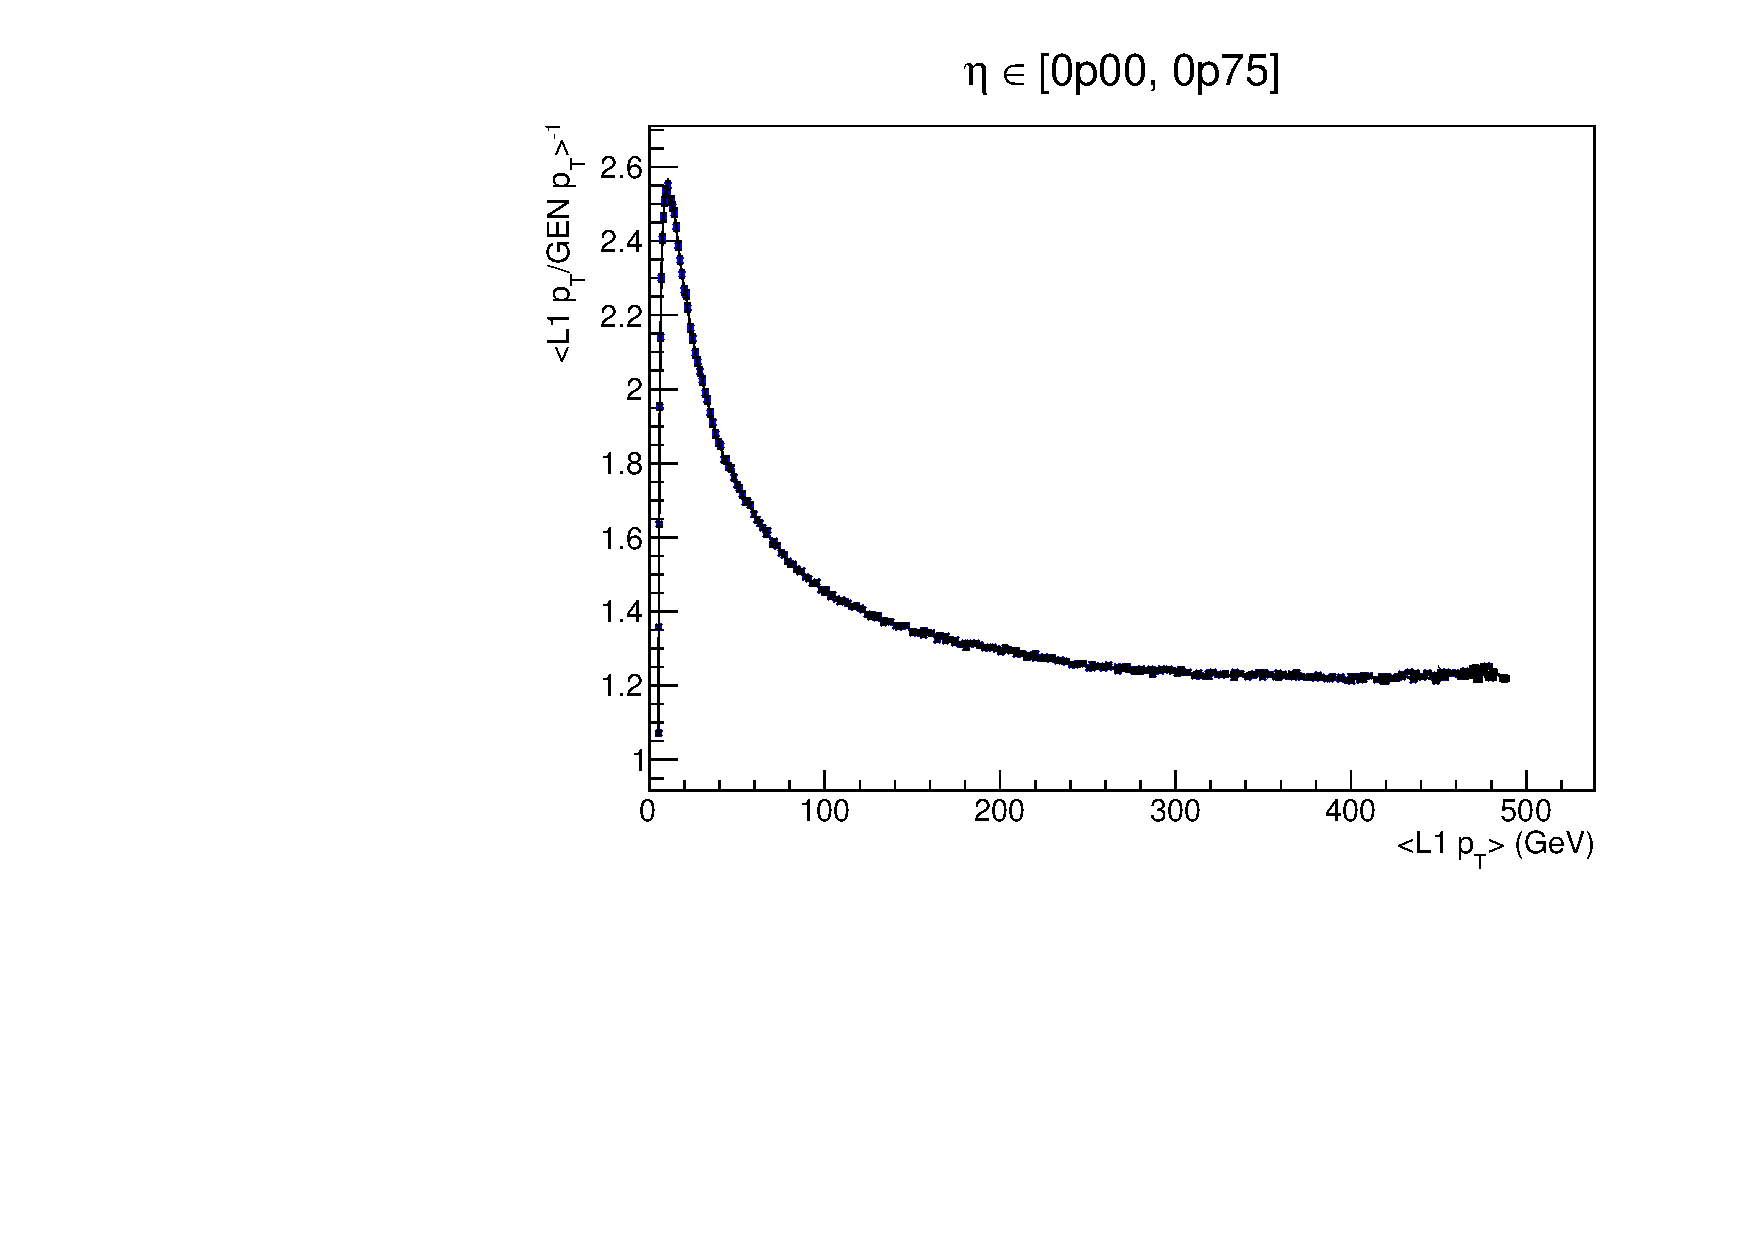
\includegraphics[width=0.8\textwidth]{./Figures/triggerUpgrade/calibrationSeed5Chunky}
  \caption{
  Fitted response for a QCD dijet sample in the range $0. < \eta < 0.75$ }
  \label{fig:response}
\end{figure}

\begin{figure}
\centering
    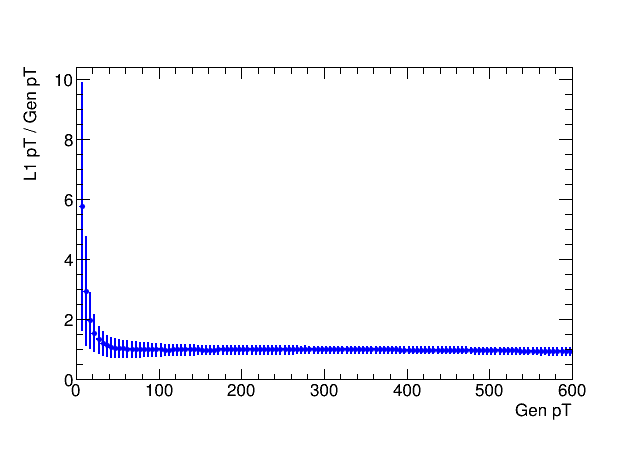
\includegraphics[width=0.8\textwidth]{./Figures/triggerUpgrade/calib_s5_chunky}
  \caption{Calibrated response in the QCD dijet sample used to derive the calibration factors. The calibration is seen to be 
  effective for the range $\Lonept > \sim 20\GeV$.}
  \label{fig:closure_response}
\end{figure}

\section{Jet performance}
\label{sec:trig_perf}
The performance of the jet algorithm and the various pileup suppression techniques is tested using
MC simulations. In each case the $\Lonept$ is calibrated following the procedure in Section~\ref{sec:calib}.
Comparisons are made with algorithms used for both the legacy GCT and UCT systems to benchmark the performance.
Unless otherwise stated efficiencies are measured using a simulated top pair production sample while 
background rates are measured using a simulated minimum bias sample.

\subsection{Matching efficiency}

The matching efficiency to generator jets provides a measure of the ability of the L1 jet algorithm 
to reconstruct real jets from the hard scatter. The matching procedure is the same as that used for the calibration. 
The matching efficiency for all generator jets and the fourth leading jet is shown 
in Figure~\ref{fig:match} as a function of $\Genpt$ for several benchmark pileup suppression algorithms. 
The efficiency is seen to plateau at unity around $\Genpt=50\GeV$. The PUS and seed threshold is shown to reduce
the matching efficiency at low $p_T$, however, for this low $p_T$ region the L1 jets matched to generated jets are typically
reconstructed from pileup calorimeter deposits rather than those from the hard scatter and their energy does not 
reflect that of the matched generated jet. A substantial improvement in efficiency over the GCT is observed in 
matching the fourth leading jet.


% The matching efficiency does not fully describe the performance as L1 jets matched to generated jets may be reconstructed
% from pileup energy deposits. The resolution is observed to plateau at unity for $\Genpt > \sim30\GeV$.


%%WOULD LIKE PLOT HERE!!

\begin{figure}
\begin{center}
\subfigure[All jets\label{fig:label:alljet}]{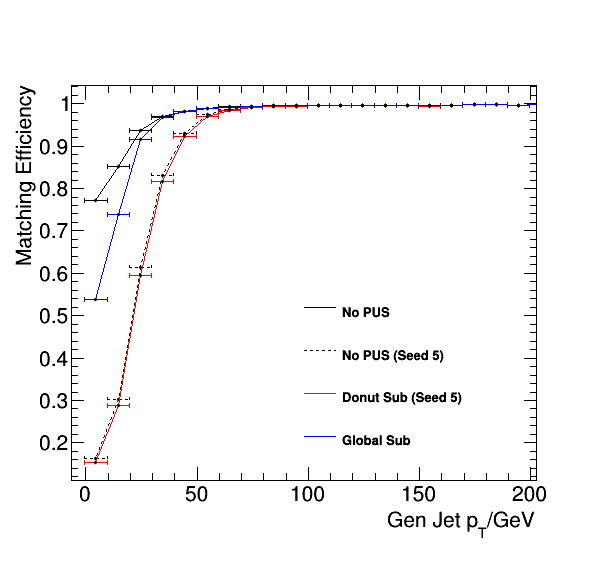
\includegraphics[width=0.4\textwidth]{./Figures/triggerUpgrade/alljet}}
\subfigure[4th jet\label{fig:label:jet4}]{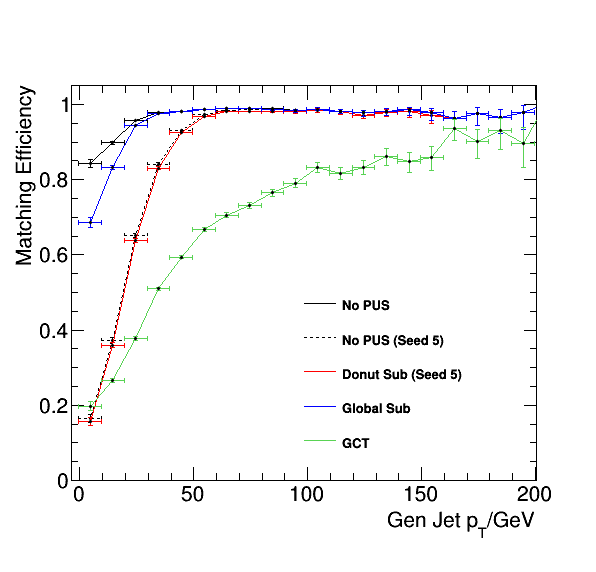
\includegraphics[width=0.4\textwidth]{./Figures/triggerUpgrade/jet4}}
\caption{Matching efficiencies for jets showing effect of seed and PUS at low energies. In \ref{fig:label:jet4} 
a comparison with the GCT is shown.}
\label{match}
\end{center}
\end{figure}

\subsection{Resolution}

The resolution, defined as $(\Lonept-\Genpt)/\Genpt - 1$, measures the agreement between the energies of the 
L1 and matched generator jets. The matching procedure is the same as that described in \Section~{sec:calib}.
The resolution provides an important measure of the ability of the algorithm to reject jets from pileup
energy deposits as well as to remove the contribution of pileup from real jets from the hard scatter.
In Figure~\ref{fig:resolution1}, the resolution as a function of the number of simultaneous interactions is shown for
a simulated top pair production sample. The resolution is flat near unity when PUS is applied,
but exhibits a strong dependence on pileup if uncorrected. To illustrate the pileup contamination for different
\Genpt~jets, a linear fit to the resolution as a function of pileup is made in \Genpt~bins and the resultant gradients
shown in Figure~\ref{fig:resolution2}. Pileup subtraction is shown to significantly reduce the 
pileup dependence of the resolution across $\Genpt$. If no PUS is applied, the magnitude of the gradient is
particularly enhanced for low \Genpt~where pileup contamination dominates. 

\begin{figure}
    \begin{center} 
	\subfigure[\label{fig:resolution1}]{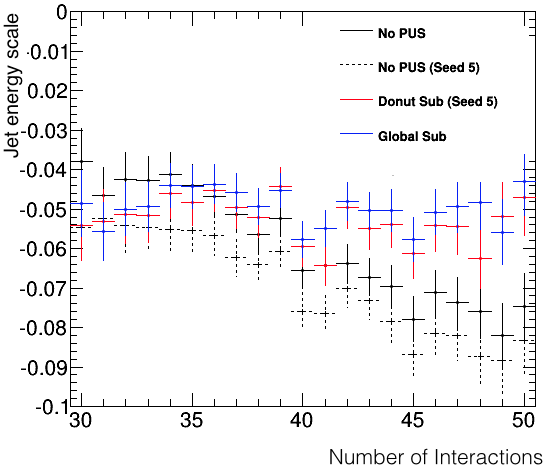
\includegraphics[width=0.5\textwidth]{./Figures/triggerUpgrade/resolution}}~
	\subfigure[\label{fig:resolution2}]{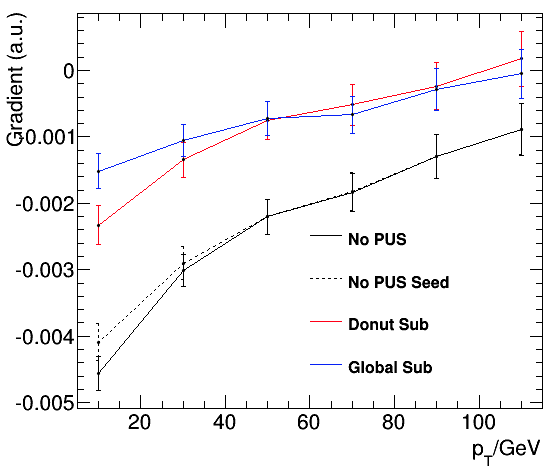
\includegraphics[width=0.5\textwidth]{./Figures/triggerUpgrade/p1eta_14to28_calib_fits}}
	\caption{(a) Resolution as a function of the number of interactions. (b) Gradients of linear fits to 
	    resolution as a function of number of interactions in bins of $p^{gen}_{T}$.}
	    \label{fig:label:resolution}
    \end{center} 
\end{figure}

\subsection{Rates and efficiencies}

The \emph{turn on} of the efficiency for generator quantities for a L1 selection of 150\GeV on the leading jet
and 100\GeV on the fourth leading jet are shown in Figure \ref{fig:turnon}. The upgrade trigger exhibits a sharper turn on
than the GCT quantities and plateaus at higher values than the legacy system. 

\begin{figure}
    \begin{center} 
	\subfigure[\label{fig:resolution1}]{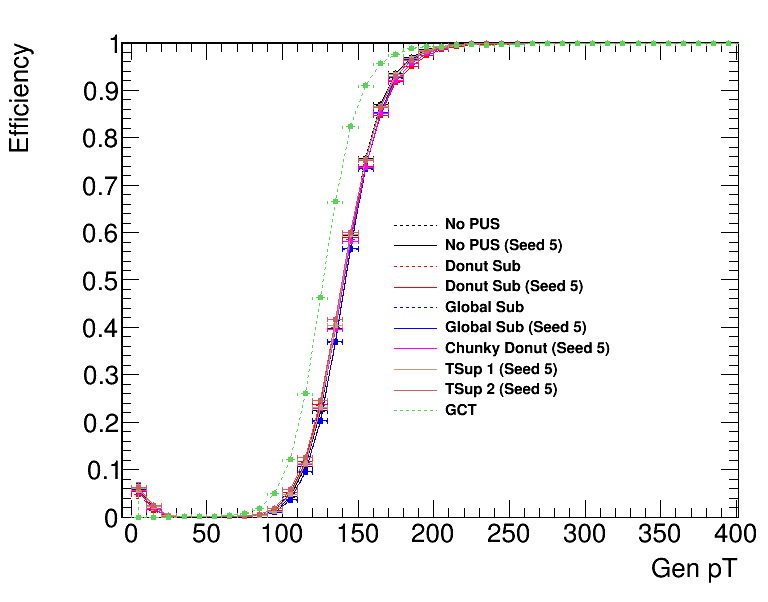
\includegraphics[width=0.5\textwidth]{./Figures/triggerUpgrade/leadJet150_noUct}}~
	\subfigure[\label{fig:resolution2}]{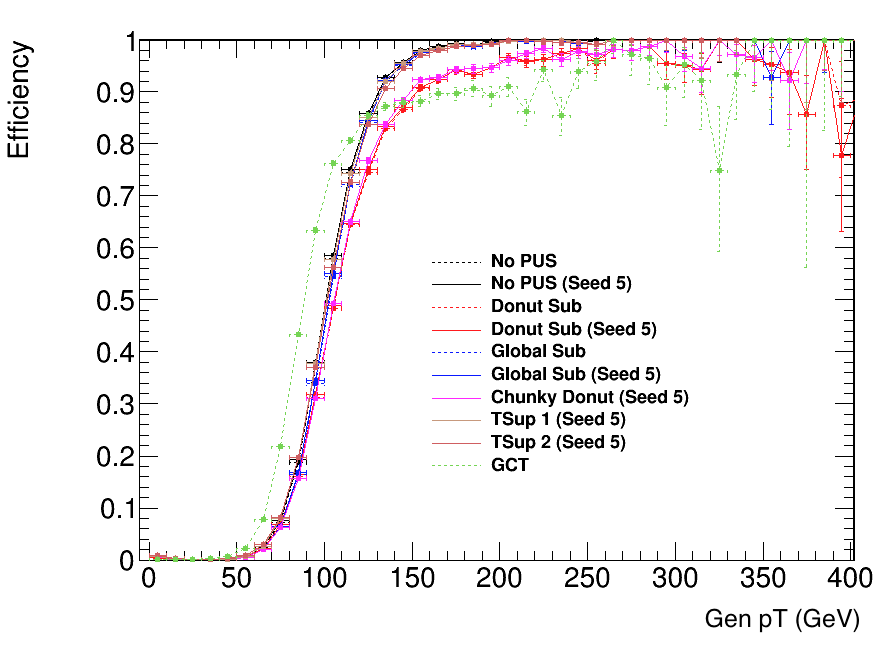
\includegraphics[width=0.5\textwidth]{./Figures/triggerUpgrade/fourthJet100_noUct}}
	\caption{Efficiency as a function of $\Genpt$ for (a) a L1 threshold of 150\GeV~on the leading jet and (b) 
	a L1 threshold of 100\GeV~on the fourth leading jet.}
	    \label{fig:turnon}
    \end{center} 
\end{figure}



The efficiencies shown in Figure~\ref{fig:turnon}, however, do not fully describe the performance 
of the trigger as the total rate of selected events must be considered and places 
stringent restrictions on the possible L1 thresholds. Figure~\ref{fig:rate_eff_jets} shows the rate of 
minimum bias events passing selection (per second) against the efficiencies for selecting 
a leading jet, second leading jet and fourth leading jet with $\Genpt$ thresholds of $150\GeV$,
$100\GeV$ and $50\GeV$ respectively. As the jet multiplicity increases and threshold decreases
the performance of the upgrade L1 jets compared to the legacy system is substantially improved.
For the upgrade L1 jets, the global $\rho$~subtraction exhibits the best performance, however, the differences 
between the PUS algorithms are small.

\begin{figure}[h!]
  \centering
    \subfigure[]{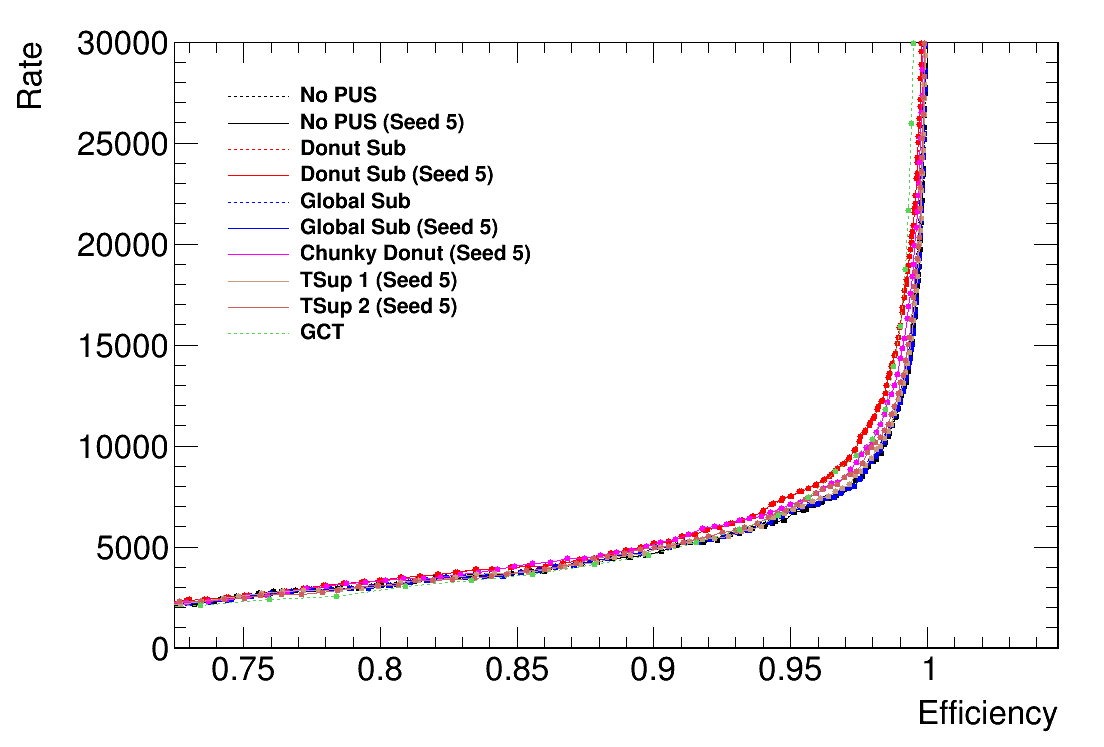
\includegraphics[width=0.4\textwidth]{./Figures/triggerUpgrade/singleJet_150.png}}~
    \subfigure[]{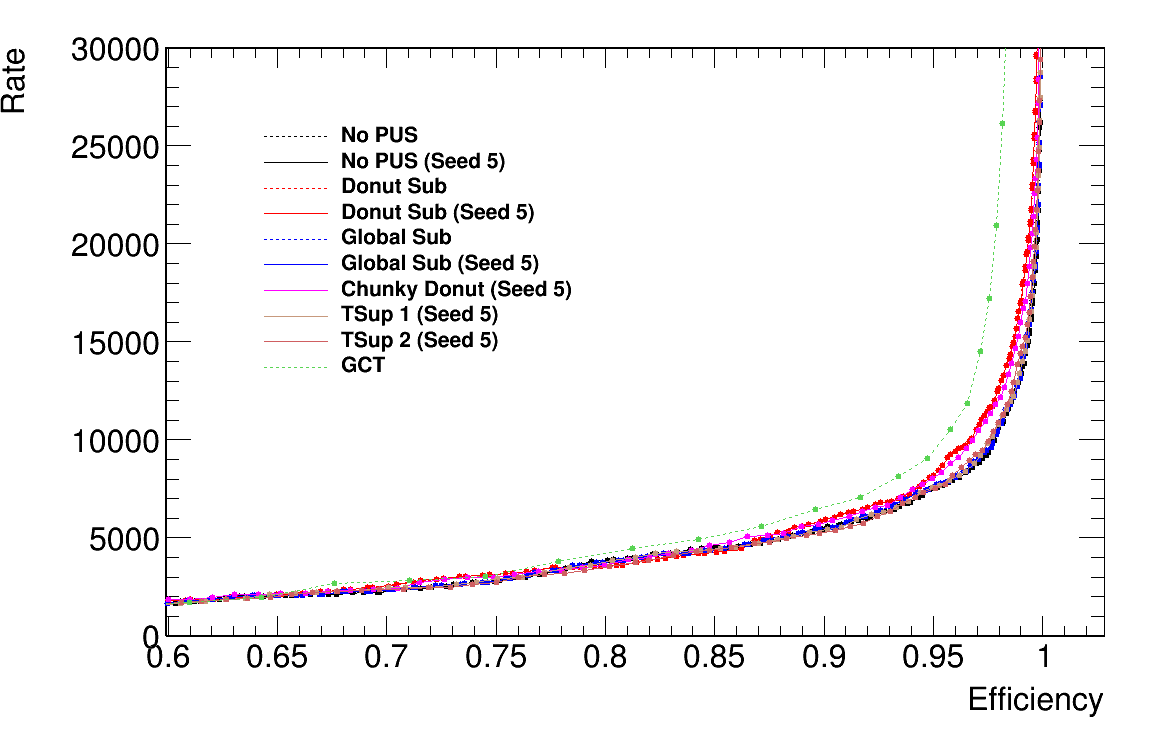
\includegraphics[width=0.4\textwidth]{./Figures/triggerUpgrade/doubleJet_110.png}}\\
    \subfigure[]{\includegraphics[width=0.4\textwidth]{./Figures/triggerUpgrade/quadJet_50.png}}
  \caption{\label{fig:rate_eff_jets} Rate against efficiency for (a) L1 leading jet with a threshold of 150\GeV, 
  (b) L1 second leading jet with a threshold of 110\GeV and (c) L1 fourth leading jet with a threshold of 50\GeV.}
\end{figure}

During Run 2 the pileup is not constant but varies with changes in instantaneous luminosity. 
Stability in the rate for different pileup scenarios is import to ensure that L1 trigger thresholds 
do not need to be increased during running. Figure~\ref{fig:rate_nvtx} shows the rate against the number of 
simultaneous interactions for a lead jet threshold of $30\GeV$. The dependence on pileup is 
seen to be significantly mitigated by chunky doughnut PUS compared to no PUS and global $\rho$
subtraction. 

\begin{figure}
\centering
    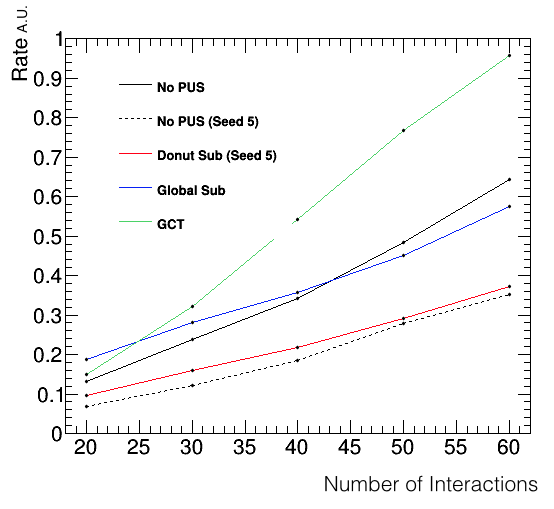
\includegraphics[width=0.8\textwidth]{./Figures/triggerUpgrade/neutrinonvtx_jet1}
  \caption{The dependence of the rate for a threshold of $\Lonept=30GeV$ on the number of simultaneous interactions}
  \label{fig:rate_nvtx}
\end{figure}

The rate against efficiency for L1 \scalht~and L1 \mht~is shown in Figure~\ref{fig:rate_eff_sum}. All jets above $20\GeV$ are
used to calculate L1 \scalht and so this quantity is particularly susceptible to pileup. The chunky doughnut 
PUS with a seed of 5 is shown to significantly improve the performance compared to the performance of other PUS
methods and the legacy system\footnote{The performance of the UCT is not 
directly comparable as L1 \scalht~and \mht are calculated using calo regions above a threshold
rather than jets} (except global $\rho$ with a seed of 5, not viable in the L1 trigger). Similarly, the performance for 
L1 \mht~is optimal for chunky doughnut subtraction with a seed of 5 and global $\rho$ subtraction. 
Figure~\ref{fig:mht_rateEff} also shows L1 $\met$~which exhibits the best performance. This is expected as 
pileup contributions are approximately uniformly deposited in $\phi$ throughout the detector and their contribution will
cancel in the vector sum of the calo towers.

\begin{figure}
\centering
	\subfigure[]{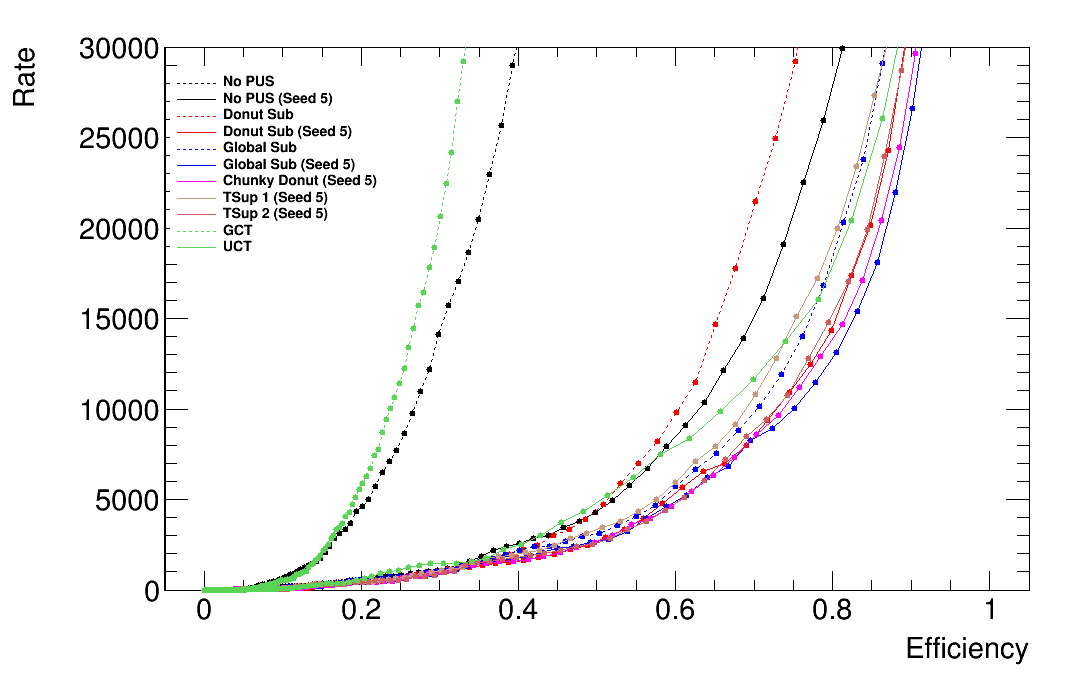
\includegraphics[width=0.5\textwidth]{./Figures/triggerUpgrade/ht_200}\label{fig:ht_rateEff}}~
	\subfigure[]{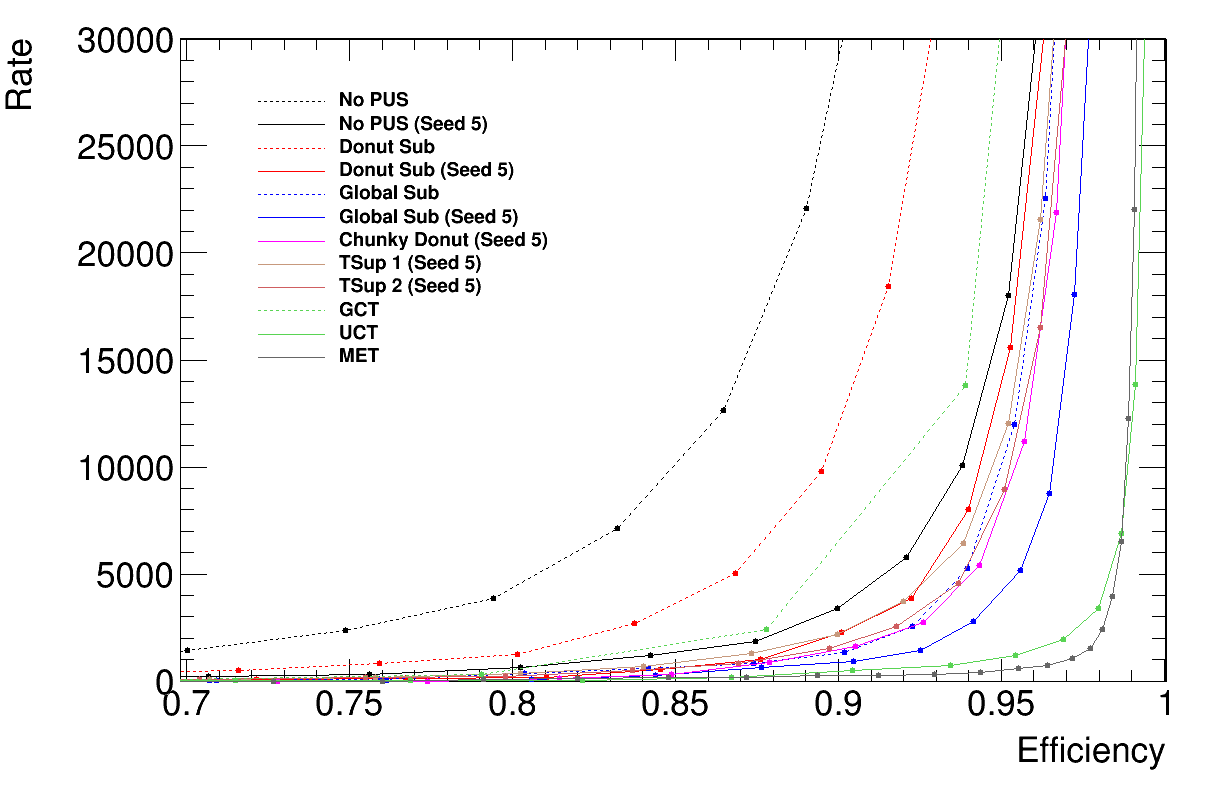
\includegraphics[width=0.5\textwidth]{./Figures/triggerUpgrade/mht_200}\label{fig:mht_rateEff}}
	\caption{Rate against efficiency for (a) L1 \scalht and (b) L1 \mht, both with a
	threshold of 200\GeV.}
	    \label{fig:rate_eff_sum}
\end{figure}

\section{Cross trigger study}

The simple single object triggers considered in the previous section are useful for selecting
high \pt~ signatures and for low luminosities. In order to provide efficiency for
the full range of the CMS physics program at higher luminosities, sophisticated combinations
of the single object triggers (cross triggers) are required. In this section, the \alphat 
analysis is used to highlight the utility of such a cross trigger at L1. 

The \alphat analysis is fully described in Section ??. In order to maximise the acceptance
to supersymmetric models at lower energy scales which still have reasonable missing energies
a low \scalht~threshold is required. However, without an additional requirement, the rate
would be unacceptably high. A cross trigger using a combined selection on the difference 
in $\phi$ between the two leading jets ($\Delta\phi_{1,2}$) and \scalht can control this rate while 
maintaining efficiency.

An acceptable rate for such a cross trigger, given the overall budget of 100kHz, is 
around 5.5 to 7.5 kHz. This range can be used to define a band in the plane of $\Delta\phi_{1,2}$
and \scalht~in which the efficiency can be inspected. To avoid signal model dependence, the 
efficiency is measured using a \ttbar sample for the multijet case ($\nj \ge 4$) and a sample  
of Z boson production in association with jets where the Z decays to neutrinos for the 
dijet case ($\nj == 2$). An hadronic selection with reconstructed (offline) $200 < \scalht < 300$ 
and $\alphat > 0.65$ is made in defining the efficiency (see Section ??). This approximates to the selection
of the lowest \scalht regions used in the \alphat~search for which achieving reasonable efficiencies is most challenging.
The results are shown for both the upgrade and UCT trigger in Figures~\ref{fig:dijet_cross} and~\ref{fig:multijet_cross} 
for the dijet and multijet trigger respectively. For the upgrade trigger, chunky doughnut corrected, calibrated jets are used.

\begin{figure}
\centering
	\subfigure[Upgrade trigger]{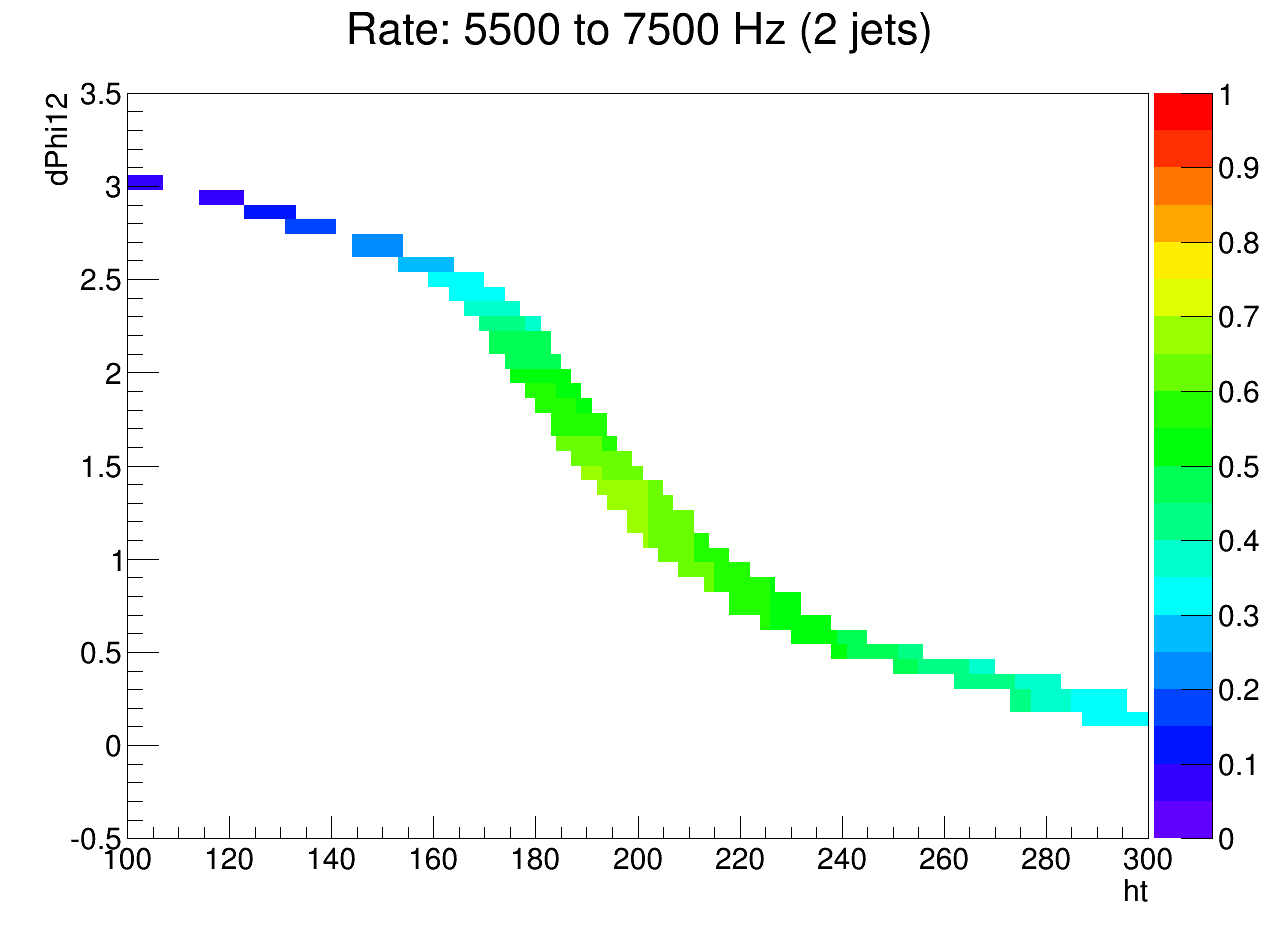
\includegraphics[width=0.5\textwidth]{./Figures/triggerUpgrade/noHardBin12JetdphiFullS2}\label{fig:ht_rateEff}}~
	\subfigure[UCT]{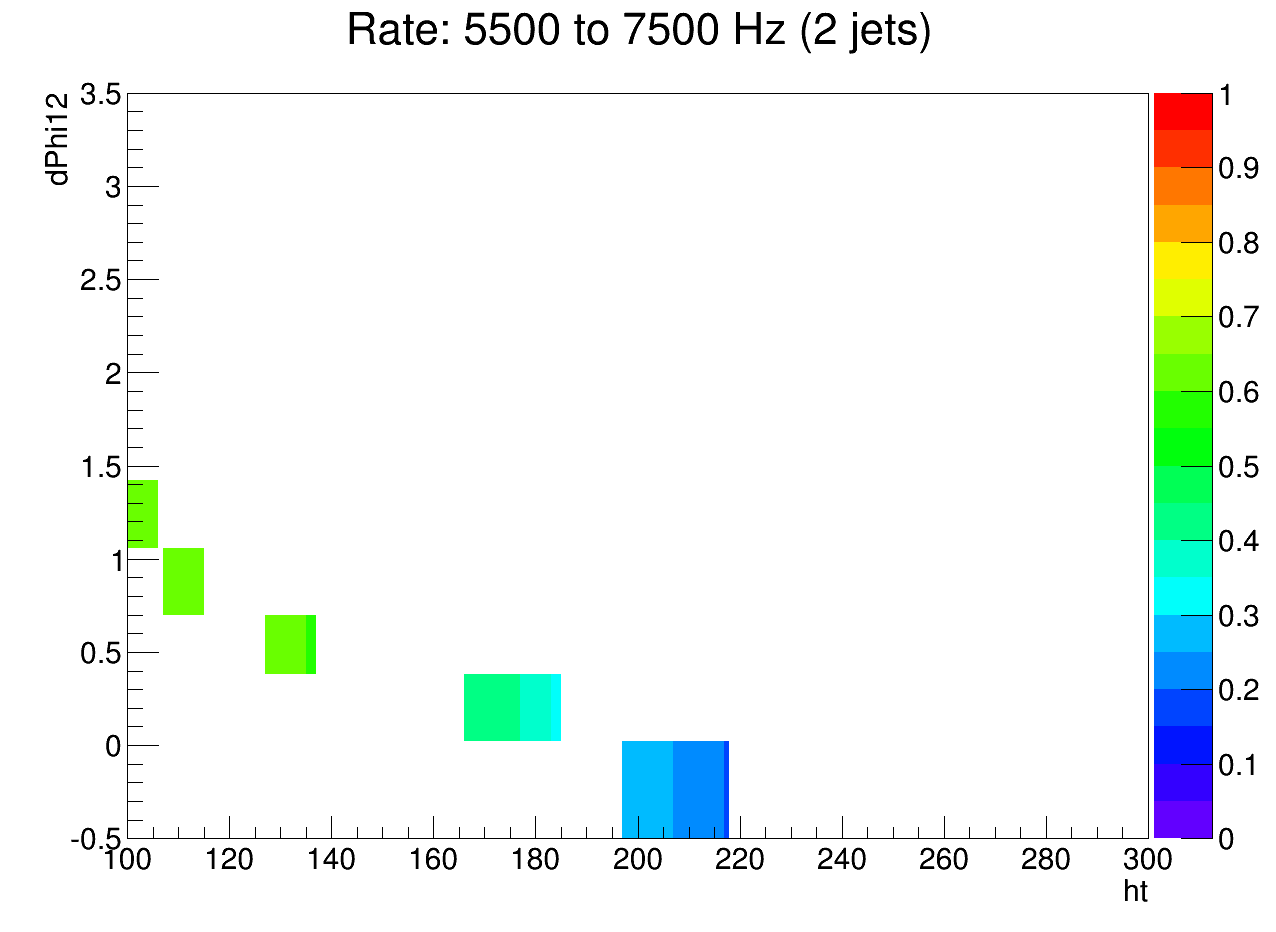
\includegraphics[width=0.5\textwidth]{./Figures/triggerUpgrade/noHardBin12JetdphiFullUCT}\label{fig:mht_rateEff}}
	\caption{Efficiency of the dijet selection for hadronic offline requirement $200 < \scalht < 300$ and $\alphat > 0.65$
	in a band of rate of 5.5 to 7.5 kHz}
	    \label{fig:dijet_cross}
\end{figure}

\begin{figure}
\centering
	\subfigure[Upgrade trigger]{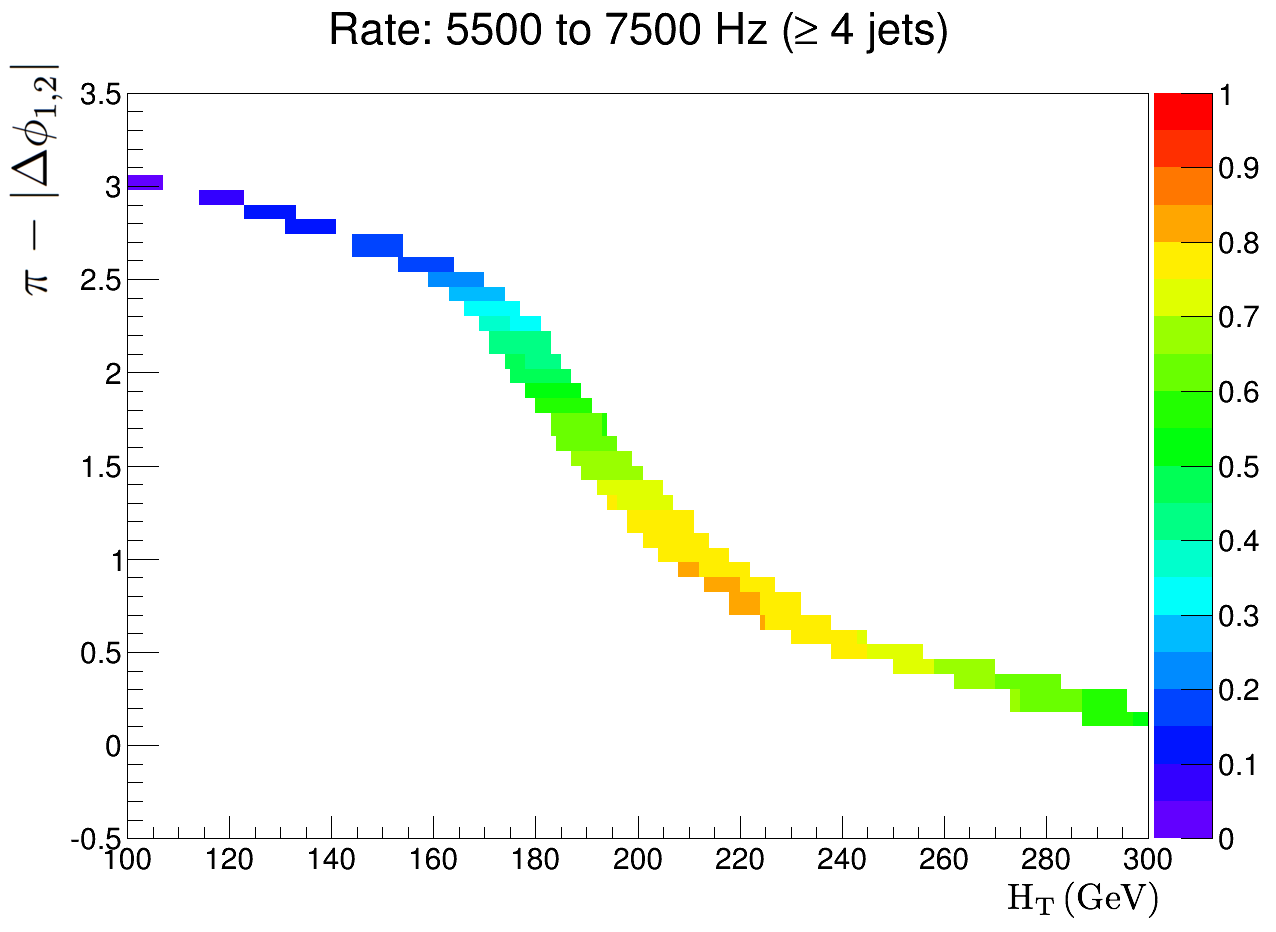
\includegraphics[width=0.5\textwidth]{./Figures/triggerUpgrade/noHardBin1ge4JetdphiFullS2}\label{fig:ht_rateEff}}~
	\subfigure[UCT]{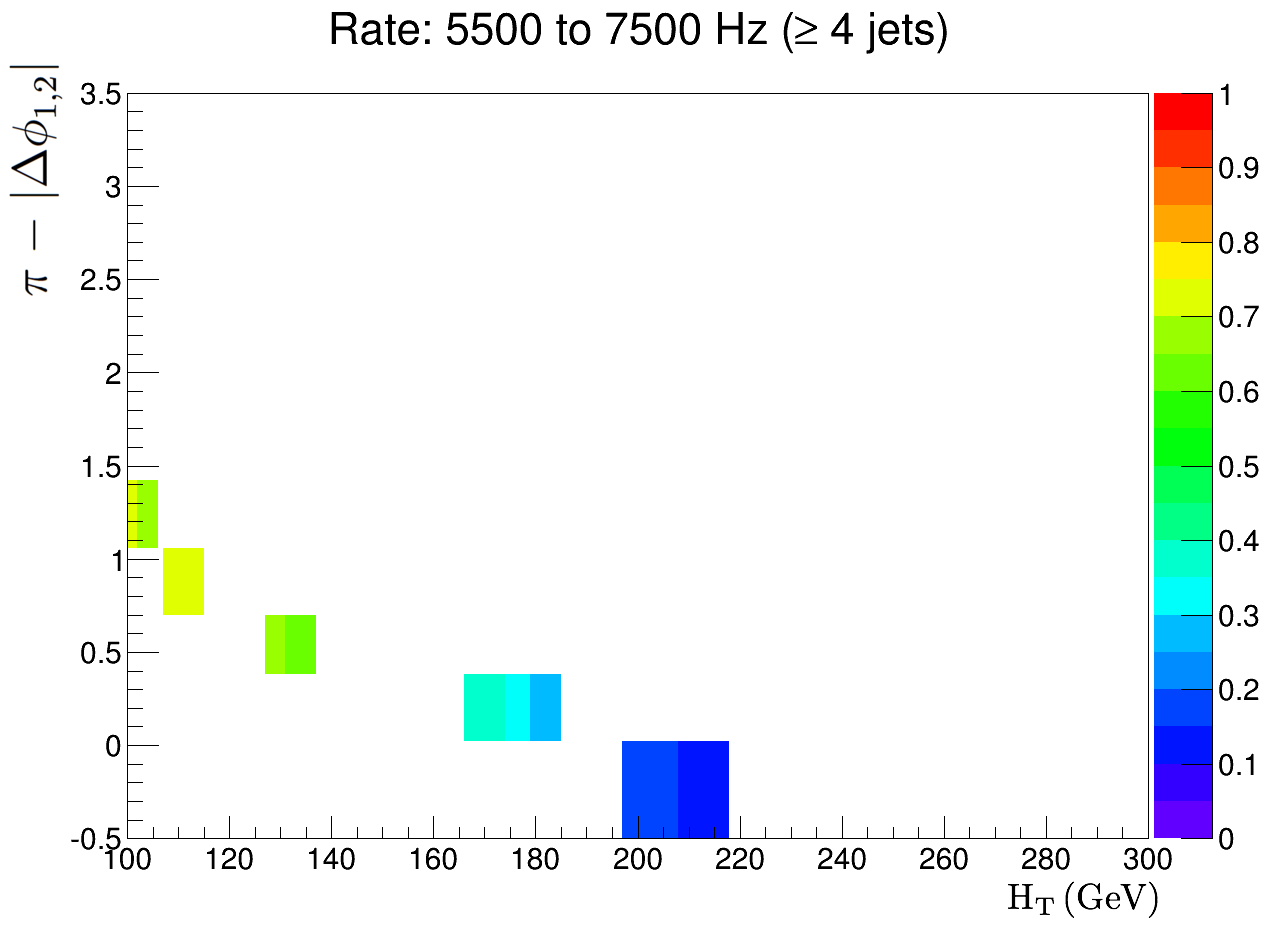
\includegraphics[width=0.5\textwidth]{./Figures/triggerUpgrade/noHardBin1ge4JetdphiFullUCT}\label{fig:mht_rateEff}}
	\caption{Efficiency of the multijet selection for hadronic offline requirement $200 < \scalht < 300$ and $\alphat > 0.65$
	in a band of rate of 5.5 to 7.5 kHz}	
	    \label{fig:multijet_cross}
\end{figure}

In both cases the greatly superior resolution afforded by the upgrade system allows a significantly
more granular operating range than the UCT. Higher efficiencies are also achievable for 
the upgraded system. Additionally, the maximal efficiency gain in using $\Delta\phi_{1,2}$ can be compared for the upgrade trigger
to that using a \scalht~trigger alone. For the dijet case there is a significant gain from $\sim 30\%$ to $\sim 70\%$, while for
the multijet the gain is from $\sim 50\%$ to $\sim 80\%$ when $\Delta\phi_{1,2}$ is used in conjunction with \scalht.
This highlights the importance of cross triggers in controlling rates while keeping low offline thresholds.
% \section{Conclusions}
%
% The jet algorithm has been shown to give very compatible 
% results with the offline anti-kT algorithm and maintain a high matching efficiency to generator level 
% quantities.  Pileup subtraction has been shown to be important for  run 2. While both global 
% and doughnut subtraction have been shown to flatten the response against number of interactions (\ref{fig:label:resolution}) 
% each has weaknesses that must be addressed. Figure \ref{fig:label:rateeff} shows that applying a seed threshold 
% is comparable to global subtraction at killing rate while maintaining efficiency. Donut subtraction appears to 
% perform less well than applying the seed threshold alone. This may be due to the 
% susceptibility to fluctuations and contamination. Further studies are underway to increase the sampling area for 
% doughnut subtraction which is expected to improve performance. Figure \ref{fig:label:sums} shows \rhoG~overestimating the 
% $H_T$. This is due to the under-subtraction bias leading to excess energy being left in 
% the event. This may be correcting by applying a seed threshold as for doughnut but 
% calculating $\rho$ using all jets. 
%
% Further studies are currently underway to utilise the $\eta$ 
% dependence of the pileup in the detector.  The seed threshold applied may be altered depending 
% on the location of the tower to further reduce rate in areas of high pileup 
% while maintaining efficiency in low pileup regions. Improving calibrations such that lower energy jets may 
% be utilised is also key. Finally, increasing the sample size to use $3\times3$ towers for 
% the seed should improve discrimination between pileup and boosted jets.

% The rate is defined as the number of 
% background events passing selection per second. The nominal rate for the L1 trigger is $\mathcal{O}100kHz$. 
% The efficiency is then the proportion of signal events which trigger. To evaluate this a 
% cut is made on the gen jets ($50GeV$). The proportion of these events with a 
% corresponding matched L1 jet over a threshold then defines the efficiency at that threshold.  For 
% the trigger, the key test is to see that the efficiency for signal may be 
% maintained while reducing the background rate. For the background a pure pileup sample was used 
% while the $t\bar{t}$ samples was used for signal. In figure \ref{fig:label:ratejet1} the rate is shown 
% for the leading jet. The performance compared to the GCT is shown to be improved. 
% The seed cut appears to have the largest effect in reducing the rate as global 
% is shown to be comparable to no pileup subtraction. Figure \ref{fig:label:ratenvtx} shows the evolution of 
% the rate with the number of interactions. GCT shows the largest dependence, as expected, while 
% for stage 2 pileup subtraction is shown to decrease this dependence. Applying doughnut subtraction appears 
% to increase the rate compared to applying a seed alone. This may be due to 
% contamination causing over subtraction. The calibration will then bring the energy above the seed. Finally, 
% in figure \ref{fig:label:rateeff} the rate is shown against efficiency for the lead jet. The seed 
% is shown to be comparable to global subtraction alone while applying doughnut subtraction worsens the 
% performance. This may again be due to contamination.
% \begin{figure}
% \centering
%     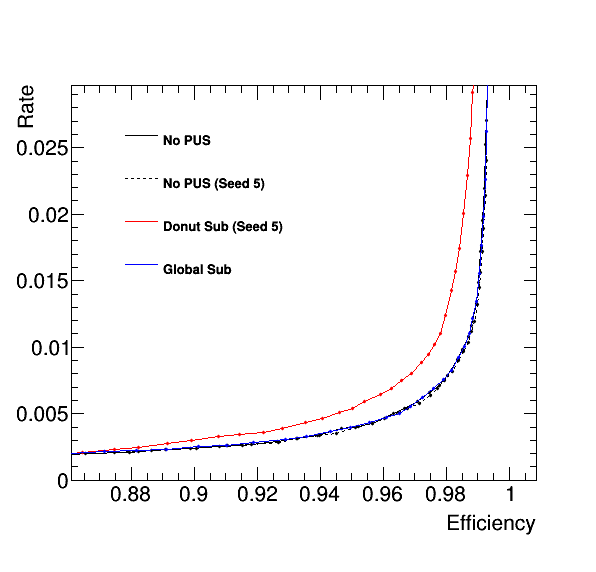
\includegraphics[width=8cm]{././Figures/triggerUpgrade/jet1RateEff}
%   \caption{Rate 
%   versus efficiency for lead jet. Performance is consistent except for doughnut which appears to 
%   excessively reduce efficiency}
%   \label{fig:label:rateeff}
% \end{figure}
% \subsection{Turn On Plots}
% To benchmark the performance of the 
% L1 jets their $p_T$ must be compared with matched generator level quantities. To do this 
% the generator level quantity is plotted with a cut on the matched L1 quantity (the 
% turn on). This is shown in figure \ref{turnon} for the 4th jet. The stage 2 
% quantities are shown to be very comparable, however, the   GCT is less sharp and thus 
% the agreement with gen worse. 
% \begin{figure}
% \centering
%     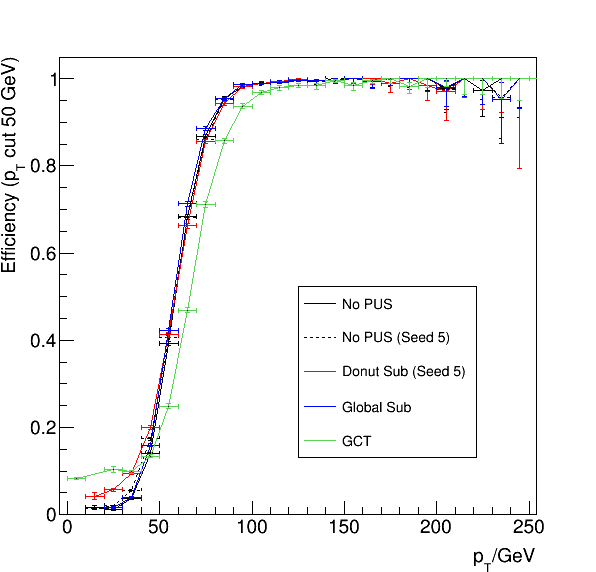
\includegraphics[width=7.5cm]{./Figures/triggerUpgrade/turnon3_50}
%   \caption{Turn on curve for the 4th jet 
%   at 50 GeV showing comparable behaviour for the stage 2 quantities and a shallower 
%   turn on for GCT.}
%   \label{turnon}
% \end{figure}
% \subsection{Energy Sums}
% Lastly, the energy sums, \scalht and 
% \mht~, were investigated. To nullify the problem of the lower calibration limit, only jets above 
% this are included in the sums. This also has the effect of removing the majority 
% of remaining clustered pileup jets. Pileup is expected to be approximately uniform and so should 
% not affect the missing energy in the event. The results for a $t\bar{t}$ sample are 
% shown in figure \ref{fig:label:sums}. Pileup subtraction improves the agreement as compared to gen.  The \scalht 
% shows especially good agreement with gen for the case of a seed as compared to 
% global $\rho$. This is due to the under subtraction bias of this method. The \mht 
% shows similar levels of agreement for all cases as expected. 
% \begin{figure}
% \hfill
% \subfigure[\scalht\label{fig:label:ht}]{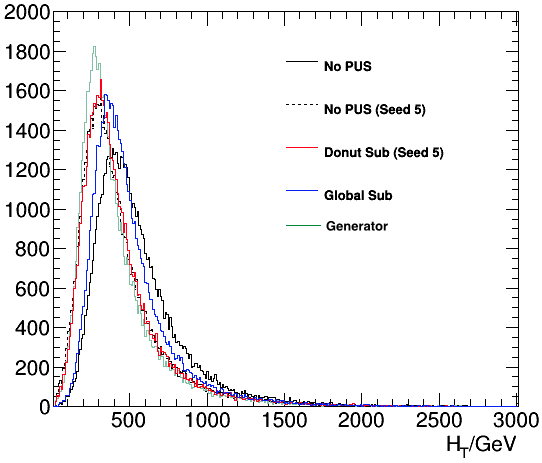
\includegraphics[width=7cm]{./Figures/triggerUpgrade/ht_ttbar}}
% \hfill
% \subfigure[\mht~\label{fig:label:mht}]{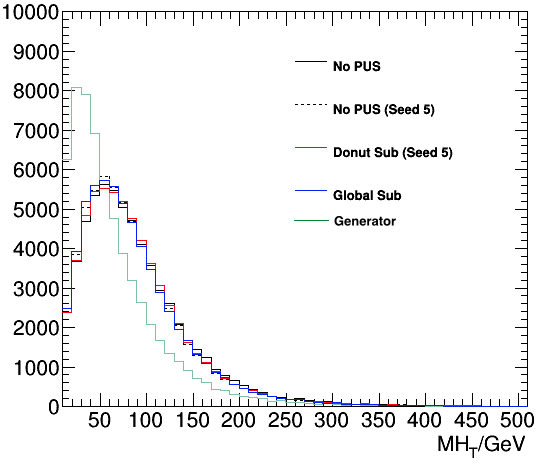
\includegraphics[width=7cm]{./Figures/triggerUpgrade/mht_ttbar}}
%
% \caption{In figure \ref{fig:label:ht} the total energy shows good agreement with the generator level quantity. This 
% is improved by requiring a seed threshold. In figure \ref{fig:label:mht} similar agreement is shown for 
% all cases}
% \label{fig:label:sums}
% \end{figure}
